\chapter{Réalisation}

\section{Introduction}
    Dans ce chapitre nous allons présenter l'environnement de développement de l'application.\\

    Nous commencerons par les techniques utilisés puis passerons vers les bibliothèques et les frameworks qui ont aidé dans cette réalisation. Par la suite, nous présenterons les outils utilisés tout le long du processus de création.\\

    Finalement, nous présenterons quelles ques interfaces de l'application.\\

\section{Présentation des technologies utilisées}
    Le but du projet est la création d'une application full-stack web. pour cela, plusieurs outils peuvent être utilisés, parmi ces outils, nous avons choisi \acs{PERN} qui est une pile de technologies conçues justement pour la création d'un environnement de développement full-stack web. \acs{PERN}, par ses initiales, se compose de PostgreSQL, ExpressJS, React et NodeJS.\\

    \acs{PERN} est un substitué de \acs{MERN}, qui est lui-même composer de MongoDB, ExpressJS, React et NodeJS. Comme \acs{MERN}, \acs{PERN} donne la possibilité de créer des applications web full-stack avec des opérations \acs{CRUD} (Create, Read, Update, Delete). Mais \acs{PERN} utilise PostgreSQL au lieu de MongoDB est nous offre un grand support pour les fonctionnalités \acs{NoSQL}, avec une forte conformité aux normes et prend en compte les transactions.\\

    \subsection{PostgreSQL\cite{postgres}}
    \begin{figure}[H]
        \centering
        
\includegraphics[scale=0.2]{ACR/postgresql.png}
        \caption{Logo de PostgreSQL}
    \end{figure}
    
    PostgreSQL est système de gestion de base de données relationnel orienté objet puissant et open-source, qui utilise \acs{SQL} et prend en charge en toute sécurité les charges de travil complexes en regroupant plusieurs fonctionnalités qui donnent priorité à l'extensibilité et la conformité.\\

    L'origine de PostgreSQL remonte a la base de données Ingres développer à l'université de la Californie de Berkley par Michael Stonebraker. Au années 1986, son créateur a repris le projet de zero est a décidé de le nommée POSTGRES, comme pour dire post-ingres. Ce n'est qu'en 1995 que son créateur à décidé d'ajouter les fonctionnalitées \acs{SQL} est a été renommée Postgre95, et ce fut qu'à la fin des années 1996 qu'il a été renommée en PostgreSQL.\\
    
    Avec plus de 30 années de développement, PostgreSQL a gagné une forte réputation grace a son architecture, sa robustesse, son extensibilité et le dévouement des contributeurs de la communauté open-source.\\

    \subsection{ExpressJS\cite{expressjs}}
    \begin{figure}[H]
        \centering
        
\includegraphics[scale=0.16]{ACR/ExpressJS-logo.png}
        \caption{Logo de ExpressJS}
    \end{figure}
    
    ExpressJS est un framework NodeJS qui fournit des fonctions puissantes pour les applications web et mobiles. Il est très simple, très léger et très flexible. Il apporte très peu de couverture et maintient le meilleur côté et une exécution rapide.\\

    En vue de son côté open source et facile d'utilisation, ExpressJS connaît une grande notoriété et possède grace aux contributeurs une grande bibliothèque de modules prêt à l'employer. ExpressJS améliore NodeJS, de façons à construire rapidement, facilement et efficacement les APIs les plus complexes.\\ 

    \subsection{React}
    \begin{figure}[H]
        \centering
        
\includegraphics[scale=0.16]{ACR/react.png}
        \caption{Logo de REACT}
    \end{figure}

    \subsection{NodeJS}

\section{Bibliothèques et Framework utilisés}
    \subsection{Axios}
    \subsection{Redux}
    \subsection{Jwt}
    \subsection{Material UI}
    \subsection{rrule}

\section{Présentation des outils utilisés}
    \subsection{Visual Studio Code}
    \subsection{Dbeaver}
    \subsection{Github}
    \subsection{Discord}
    \subsection{Lucidchart}

\section{Présentation des interfaces}
    Dans le contenu suivant, nous montrerons un aperçu du rendu final de notre application et quelle ques interfaces qui la composent.

    \subsection{Interface d'accueil}
    \begin{figure}[H]
        \centering
        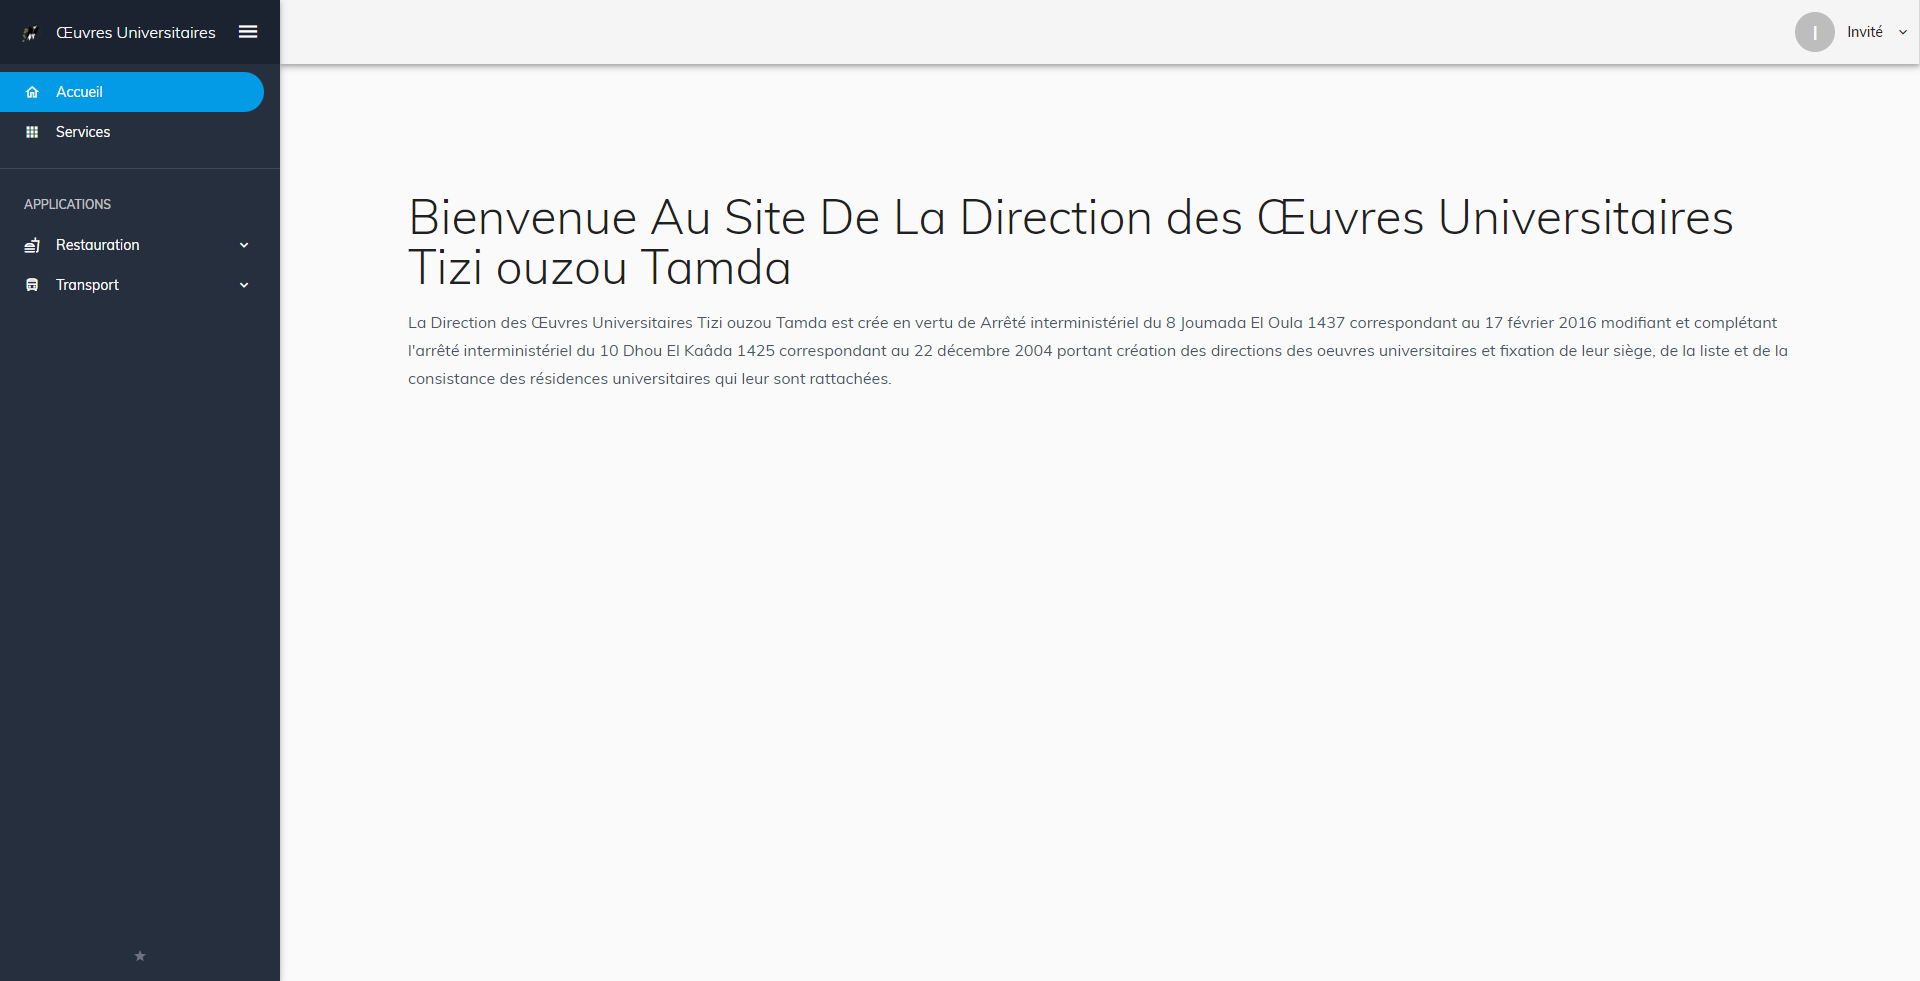
\includegraphics[scale=0.21]{PFE Screens/Invité/accueil.jpg}
        \caption{Interface d'accueil}
    \end{figure}

    \subsection{Interface d'authentification}
    \begin{figure}[H]
        \centering
        
\includegraphics[scale=0.21]{PFE Screens/Connection.jpg}
        \caption{Interface d'authentification}
    \end{figure}

    \subsection{Interface invité 'Services'}
    \begin{figure}[H]
        \centering
        \includegraphics[scale=0.21]{PFE Screens/Invité/Services.jpg}
        \caption{Interface invité 'Services'}
    \end{figure}

    \subsection{Interface invité 'Calendrier des menus'}
    \begin{figure}[H]
        \centering
        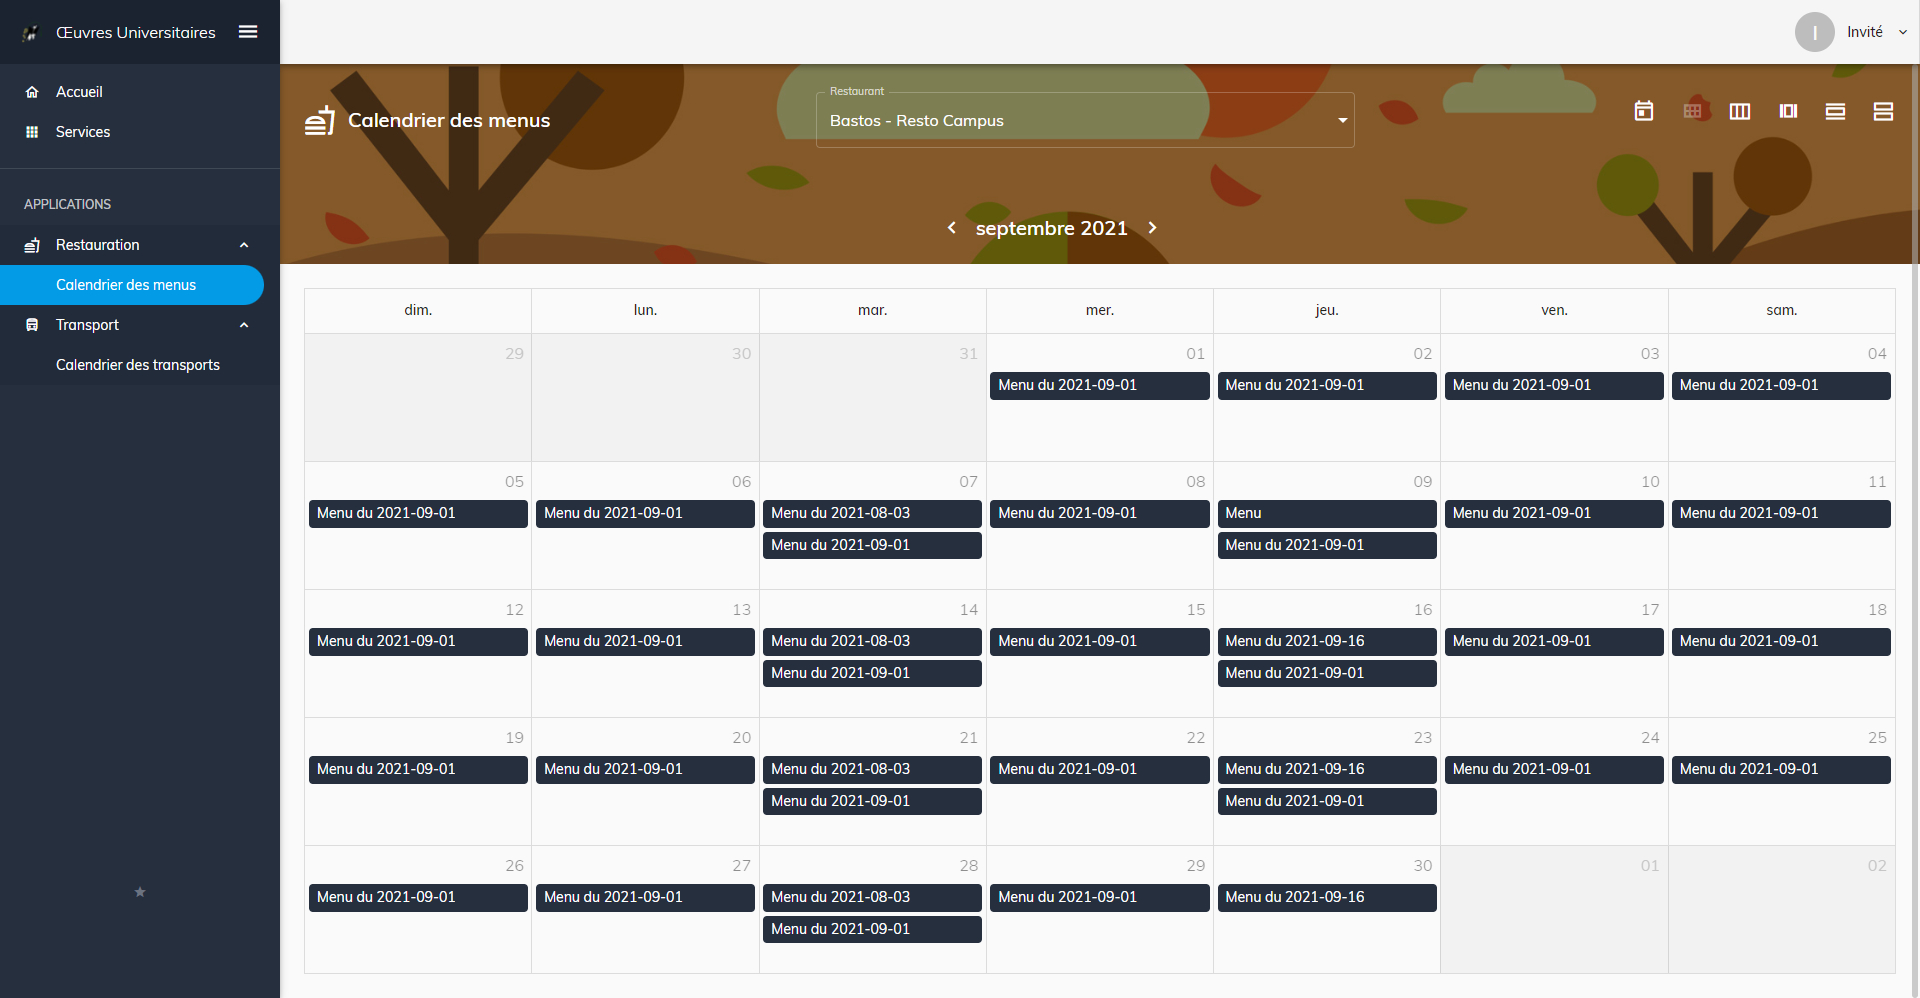
\includegraphics[scale=0.21]{PFE Screens/Invité/Restauration/Calendrier des menus.jpg}
        \caption{Interface invité 'Calendrier des menus'}
    \end{figure}

    \subsection{Interface invité 'Détail d'un menus'}
    \begin{figure}[H]
        \centering
        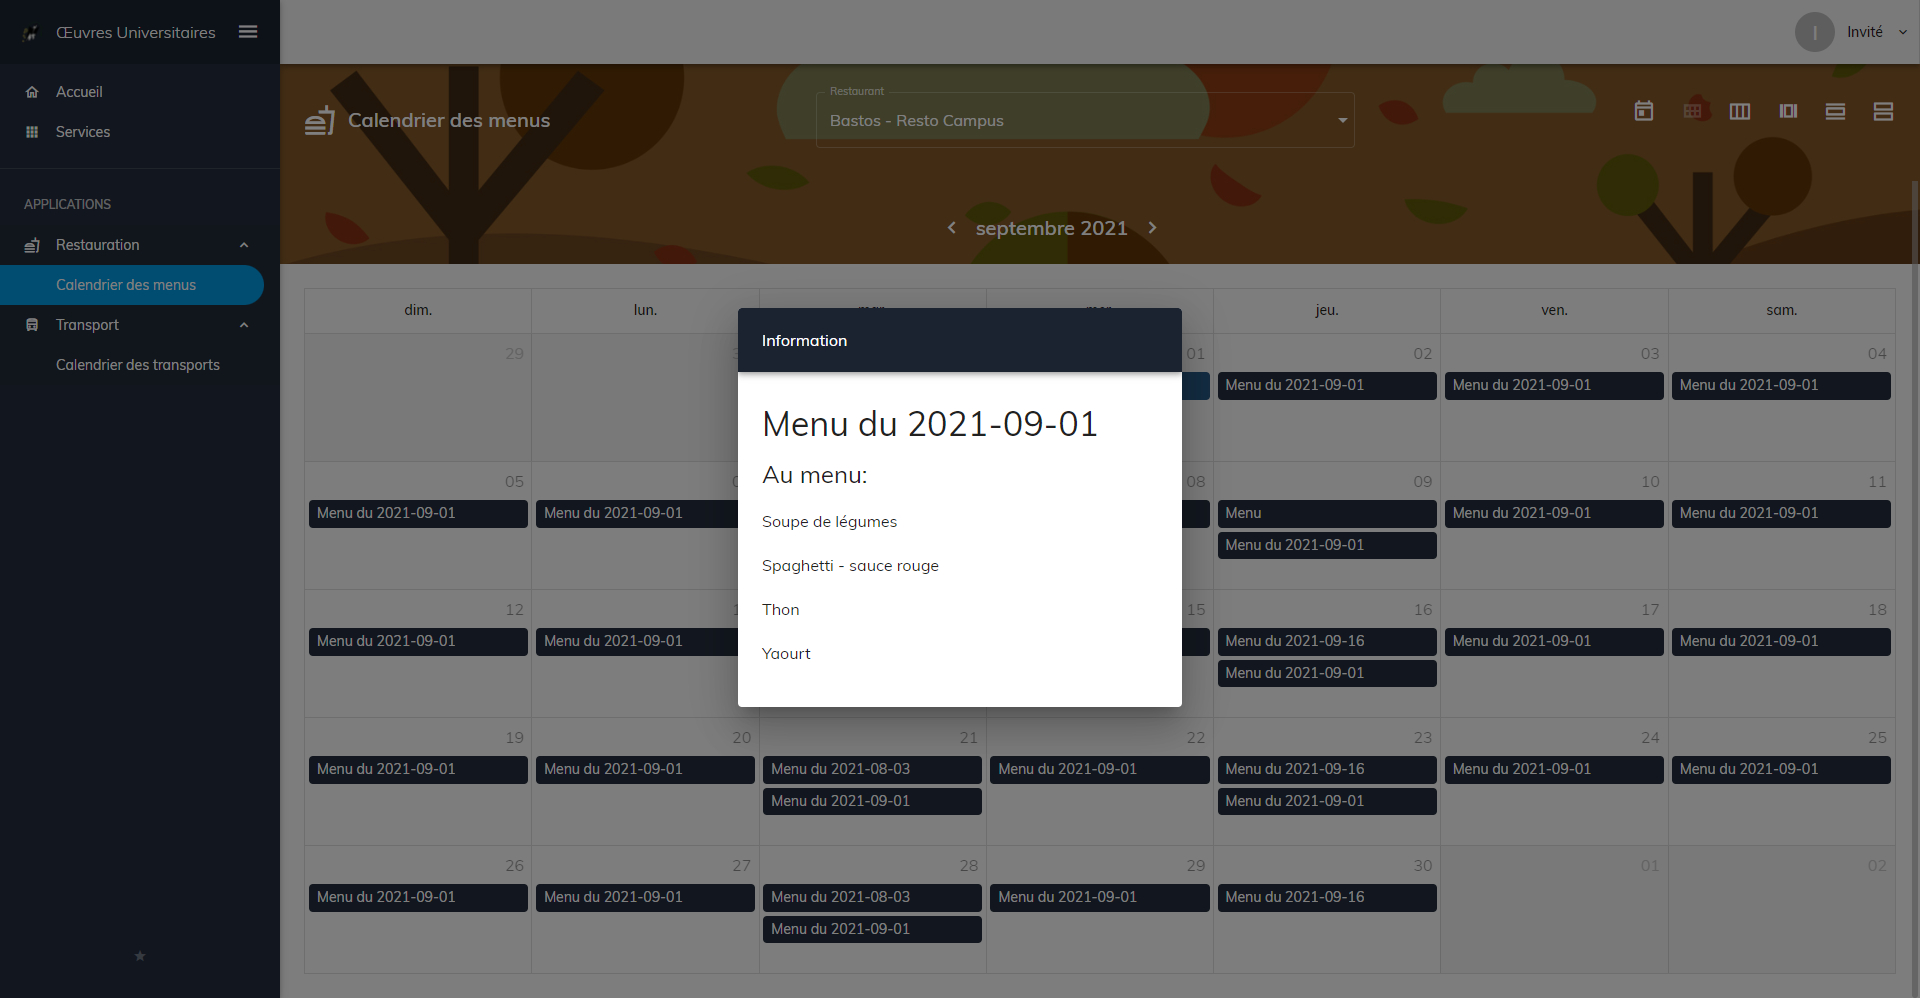
\includegraphics[scale=0.21]{PFE Screens/Invité/Restauration/Calendrier des menus - Détail.jpg}
        \caption{Interface invité 'Détail d'un menus'}
    \end{figure}
    
    \subsection{Interface d'accueil utilisateur}
    \begin{figure}[H]
        \centering
        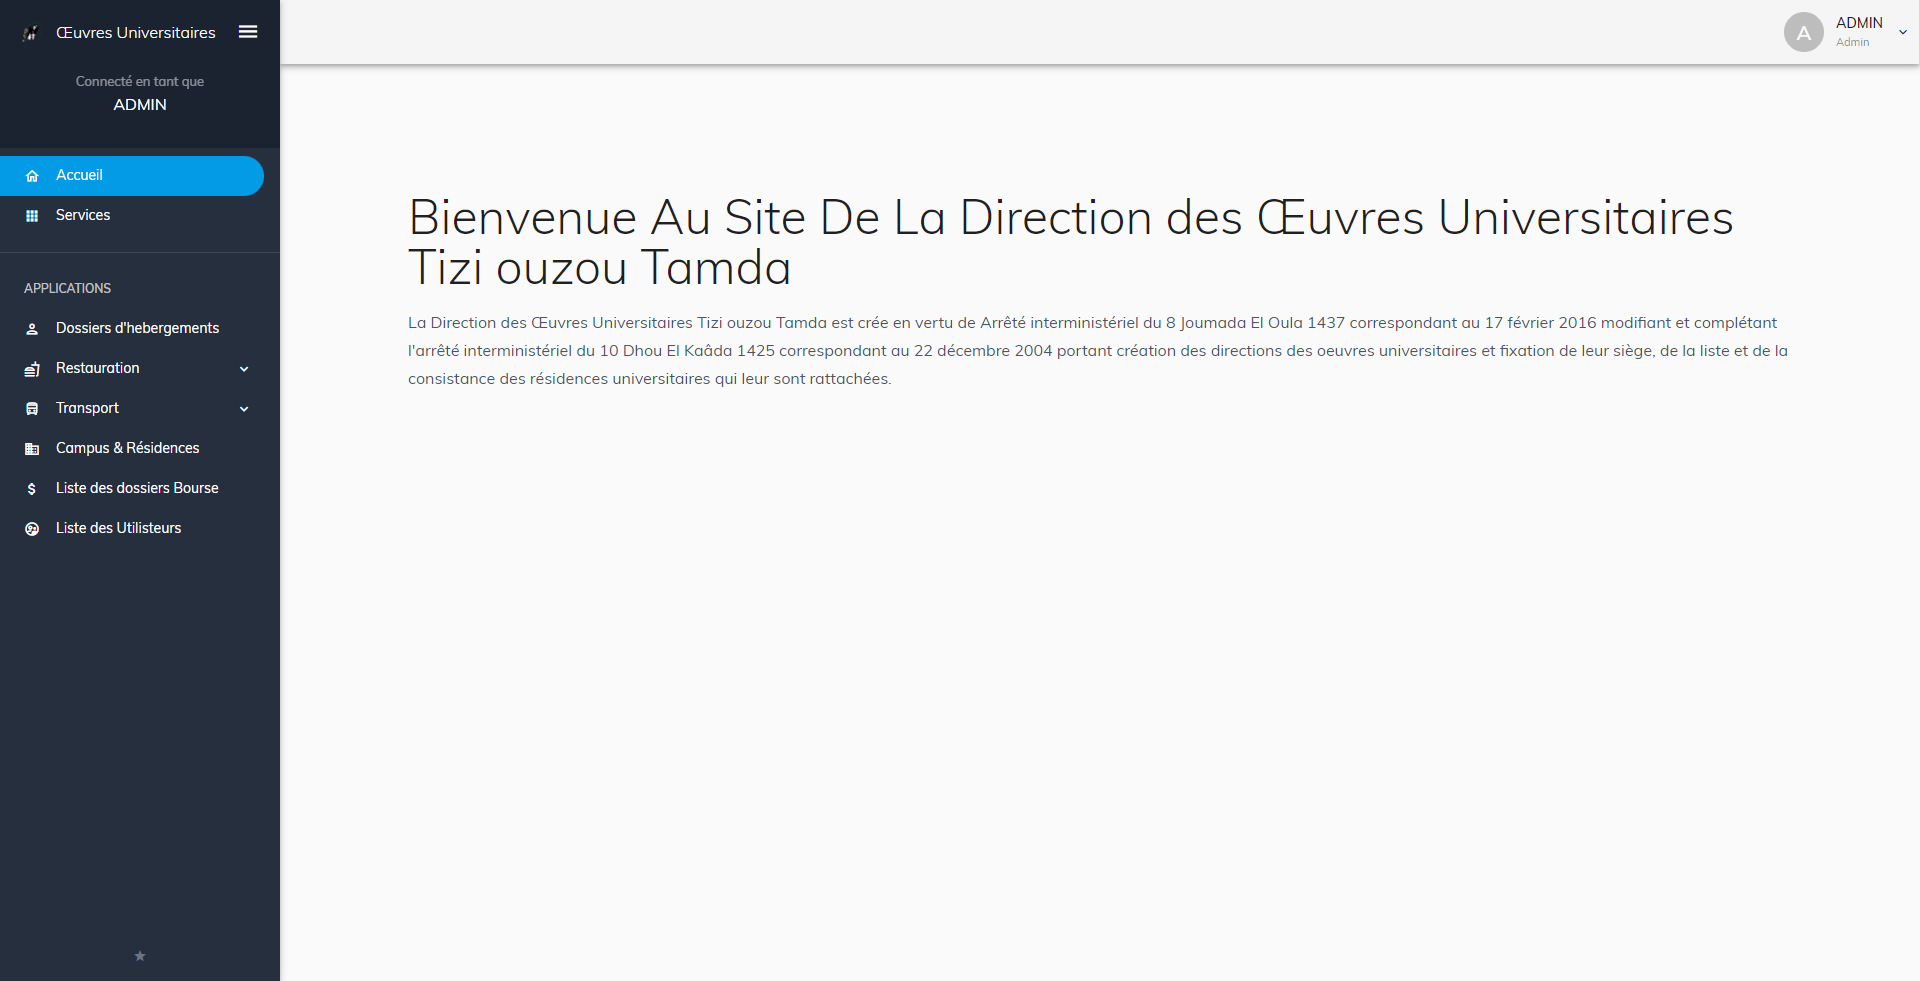
\includegraphics[scale=0.21]{PFE Screens/Admin/Accueil.jpg}
        \caption{Interface d'accueil utilisateur}
    \end{figure}

    \subsection{Interface utilisateur utilisateur 'Dossiers d'hebergements'}
    \begin{figure}[H]
        \centering
        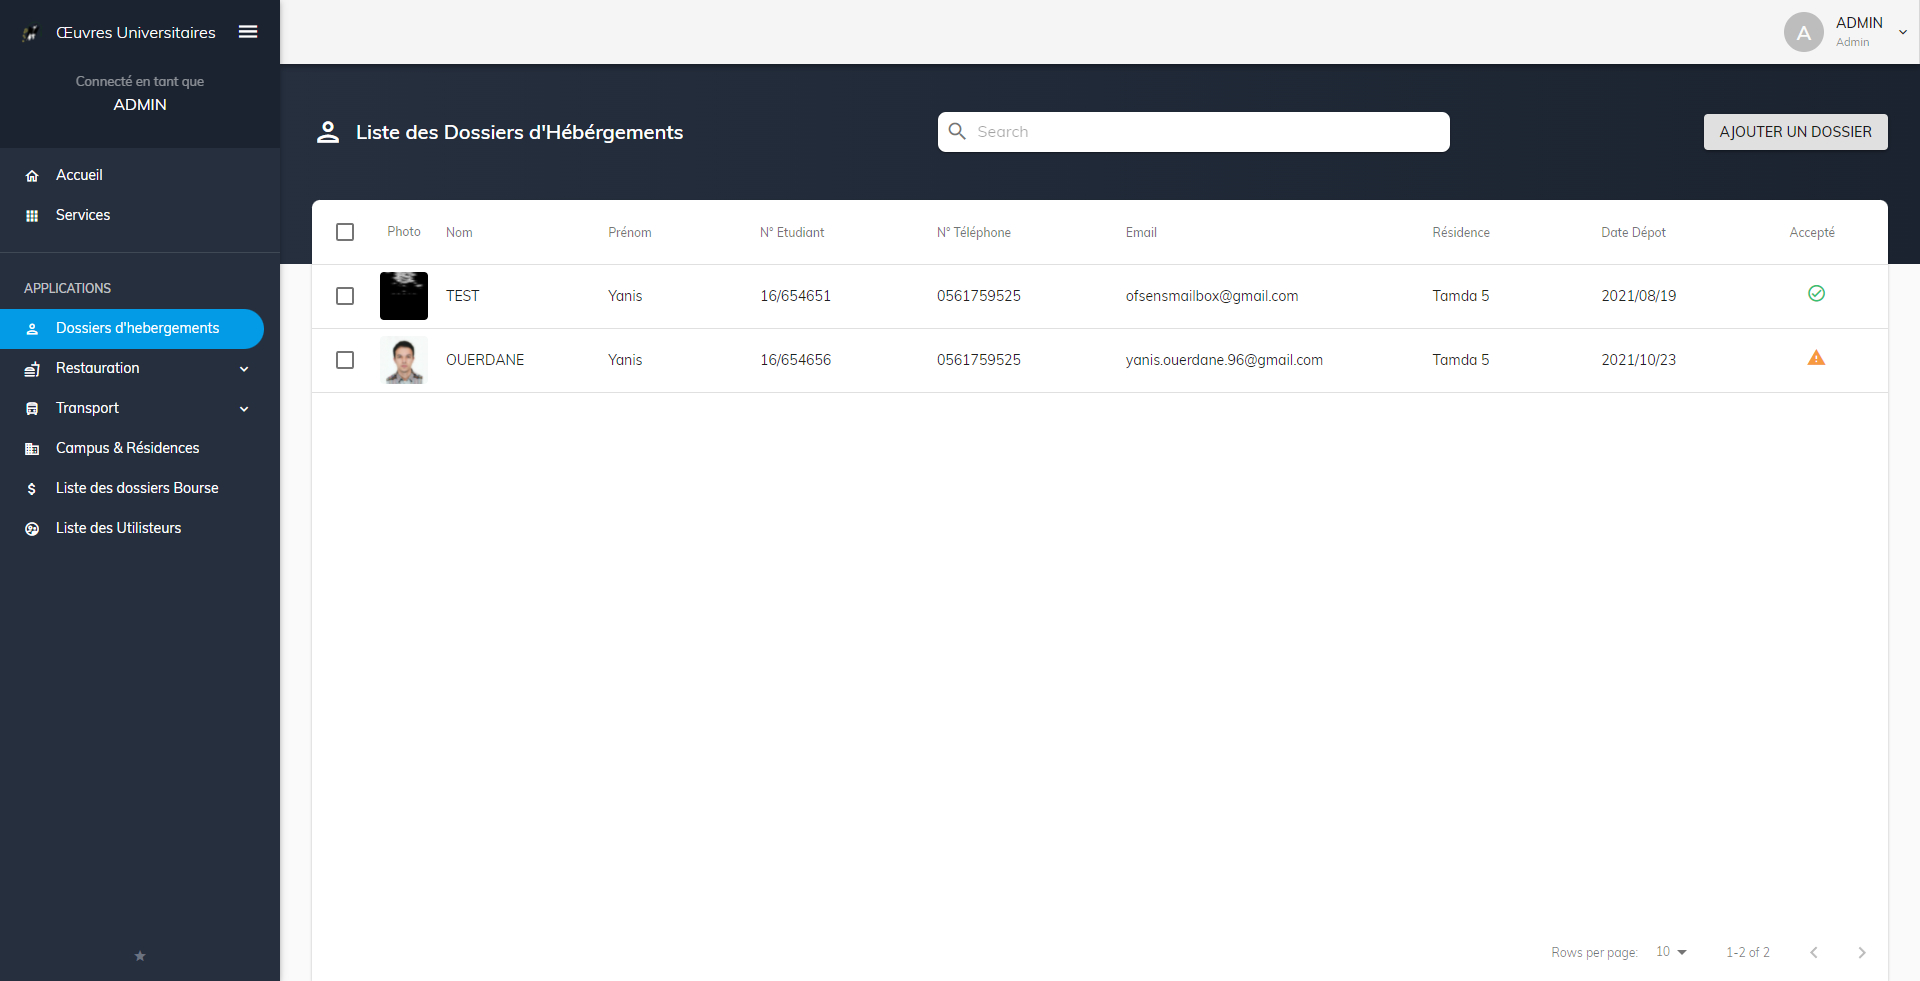
\includegraphics[scale=0.21]{PFE Screens/Admin/Hebergement/Liste des Dossiers d'Hébérgements.jpg}
        \caption{Interface utilisateur 'Dossiers d'hebergements'}
    \end{figure}

    \subsection{Interface utilisateur détail d'un dossier d'hebergements}
    \begin{figure}[H]
        \centering
        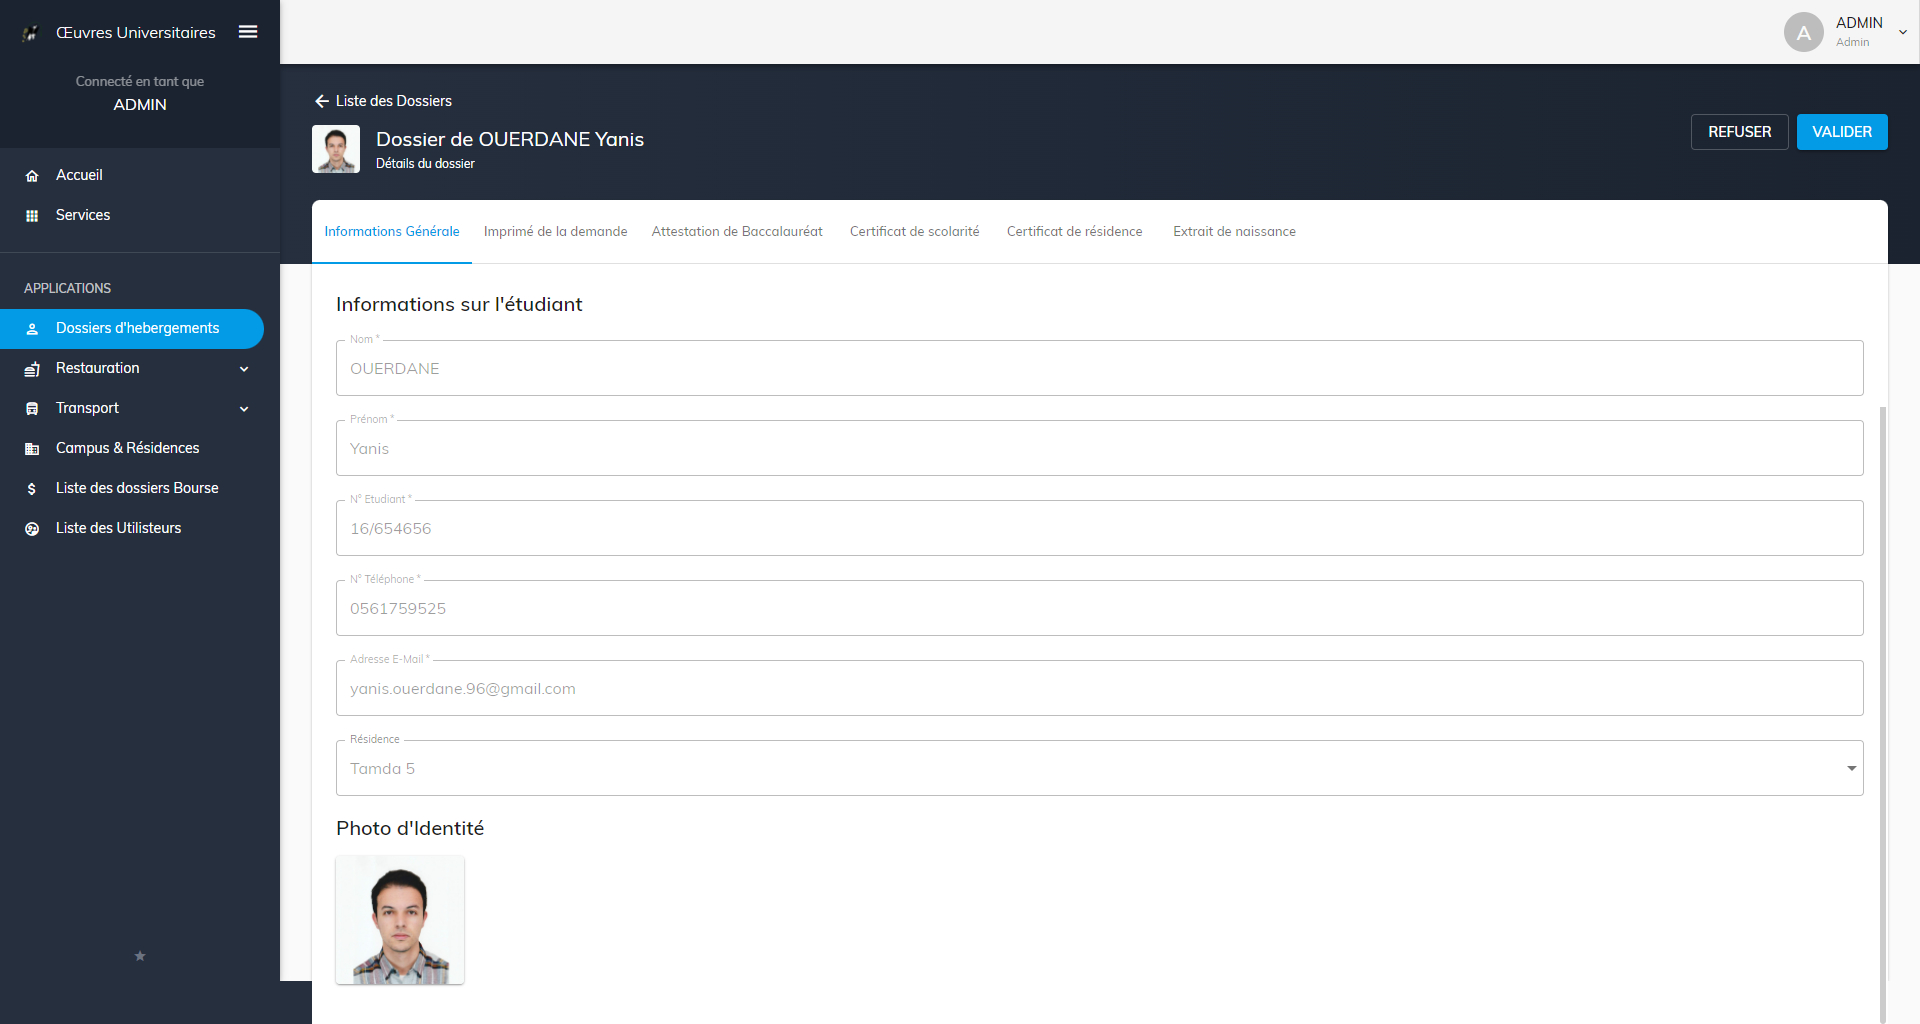
\includegraphics[scale=0.21]{PFE Screens/Admin/Hebergement/Detail.jpg}
        \caption{Interface utilisateur détail d'un dossier d'hebergements}
    \end{figure}

    \subsection{Interface utilisateur 'Liste des Réstaurants'}
    \begin{figure}[H]
        \centering
        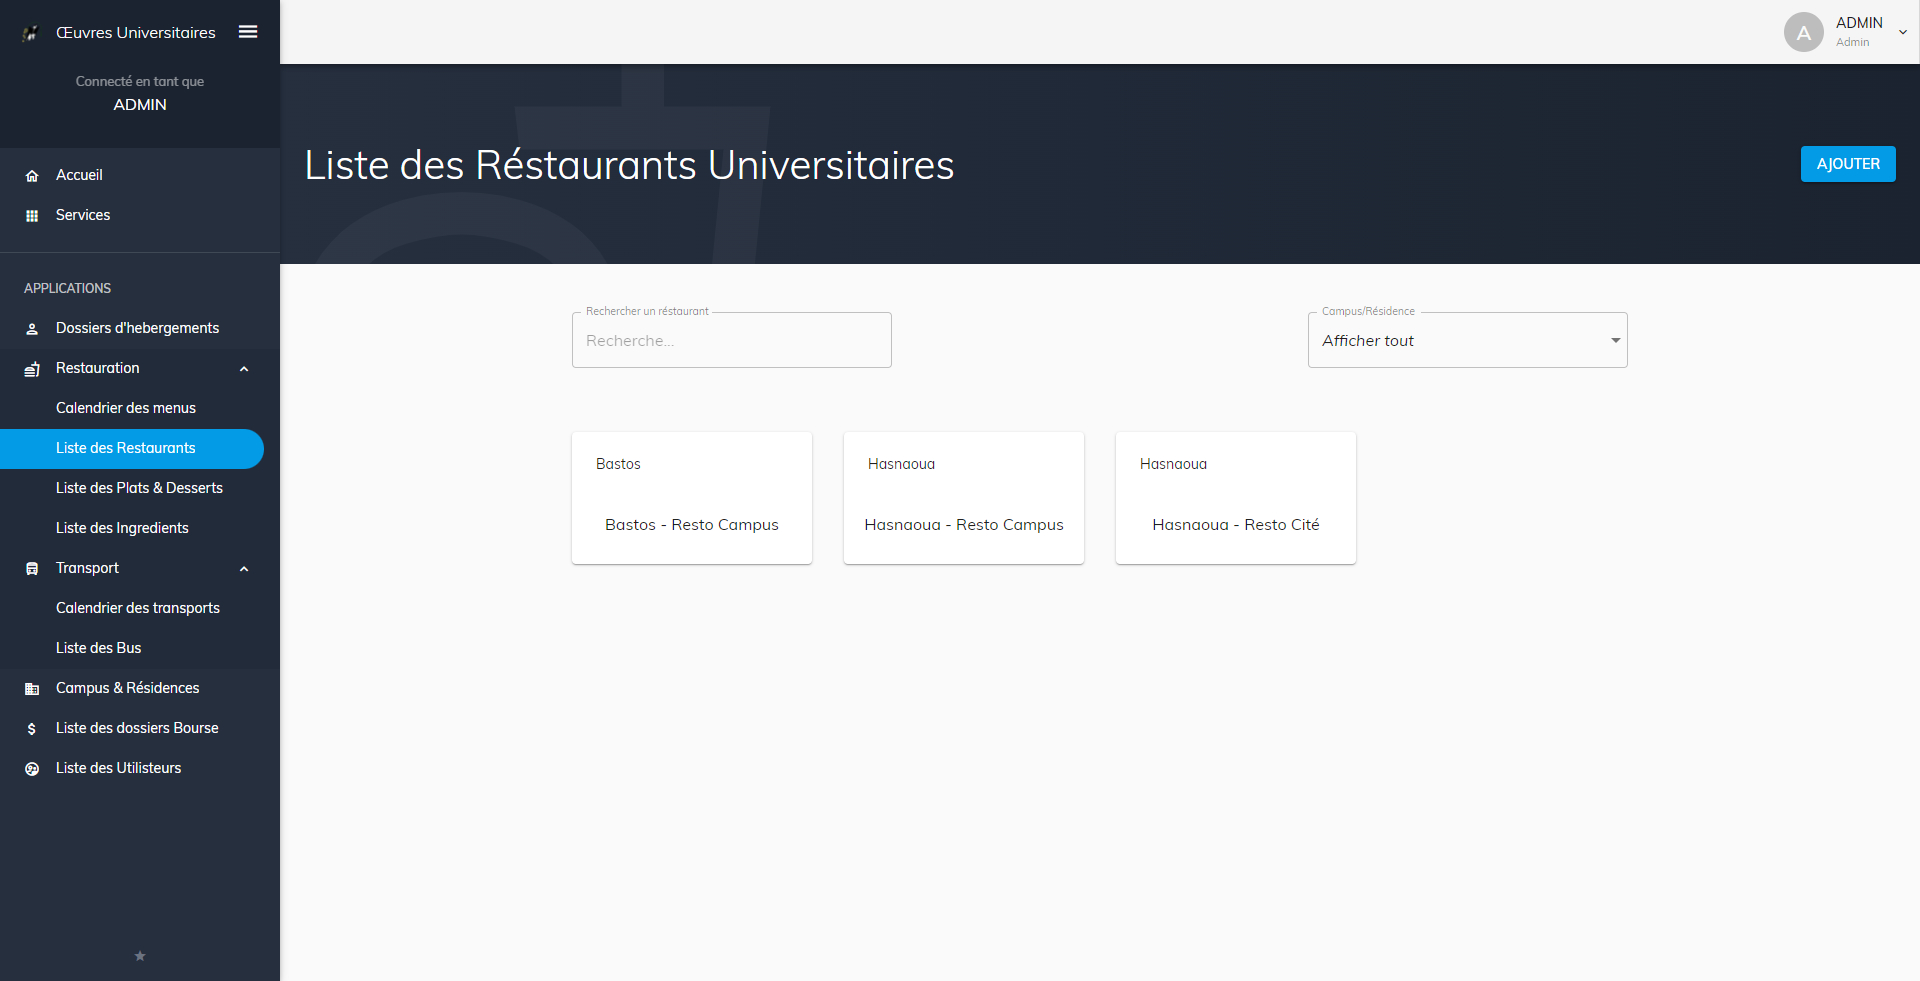
\includegraphics[scale=0.21]{PFE Screens/Admin/Restauration/Restos/Restos.jpg}
        \caption{Interface utilisateur 'Liste des Réstaurants'}
    \end{figure}

    \subsection{Interface utilisateur 'Modifier un réstaurant'}
    \begin{figure}[H]
        \centering
        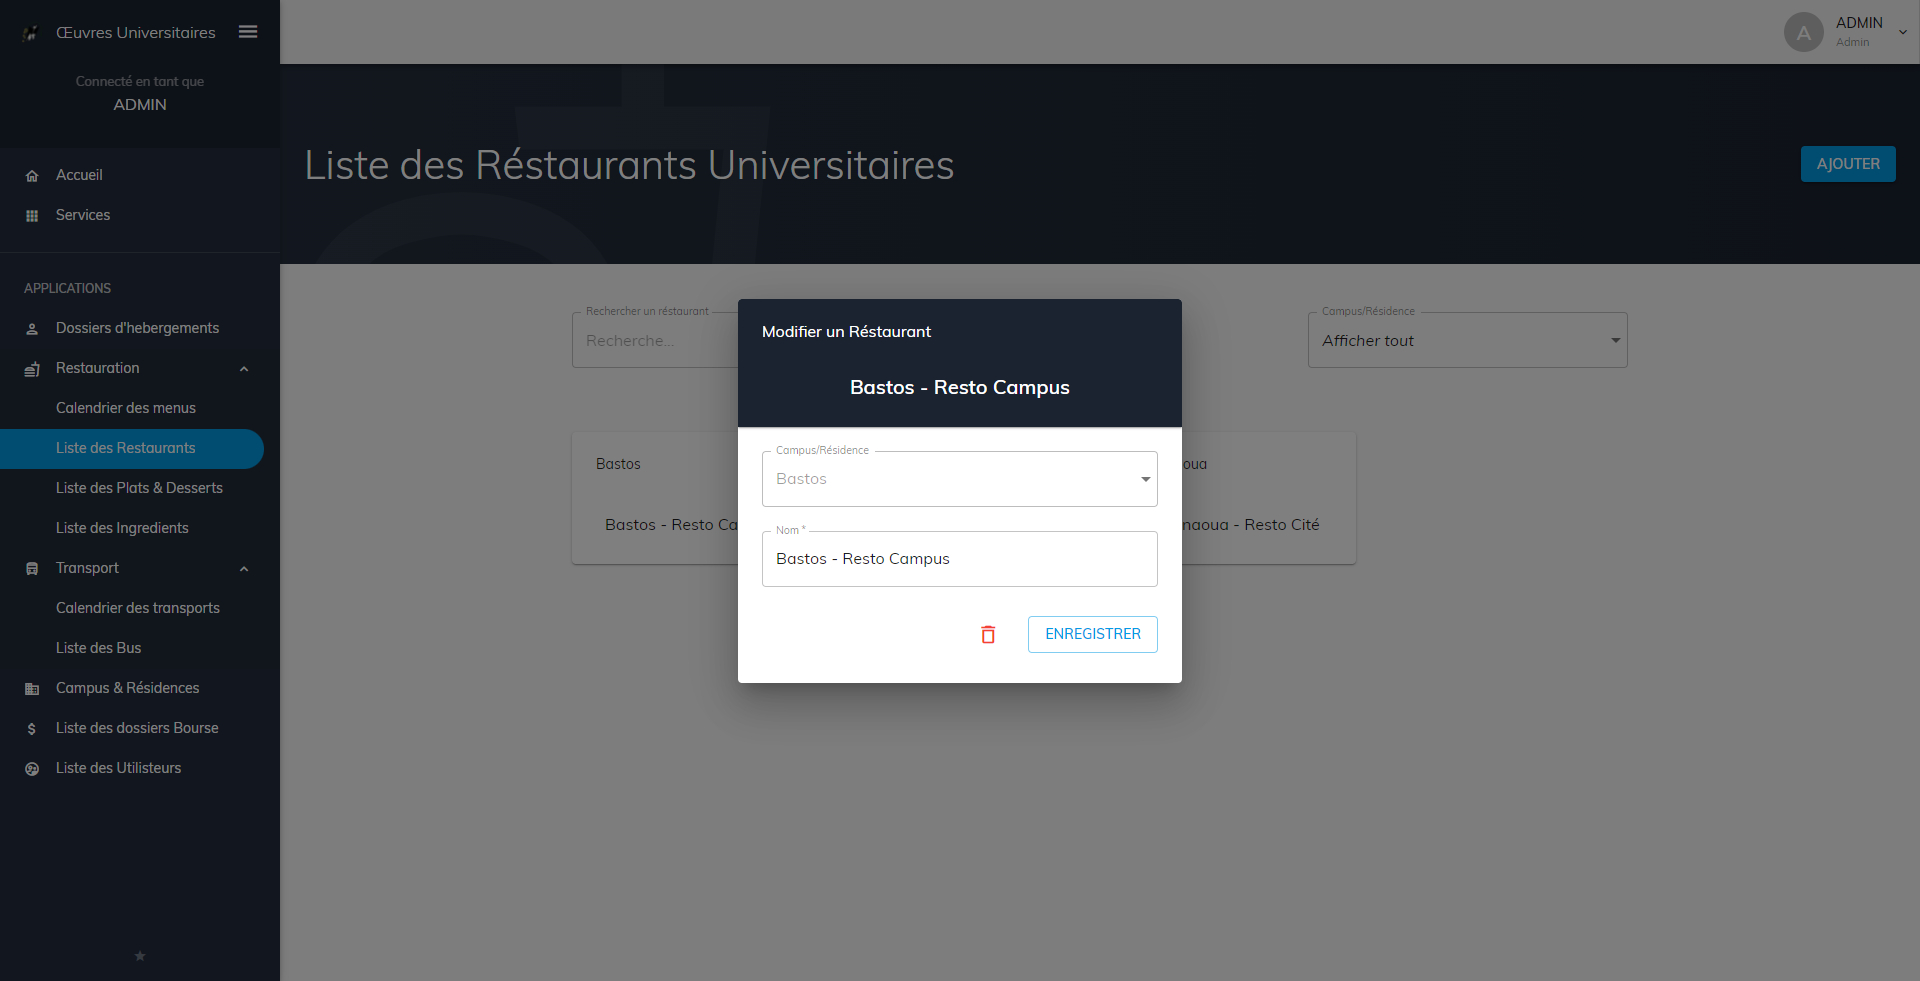
\includegraphics[scale=0.21]{PFE Screens/Admin/Restauration/Restos/Modif - Resto.jpg}
        \caption{Interface utilisateur 'Modifier un réstaurant'}
    \end{figure}

    \subsection{Interface utilisateur 'Liste des Ingredients'}
    \begin{figure}[H]
        \centering
        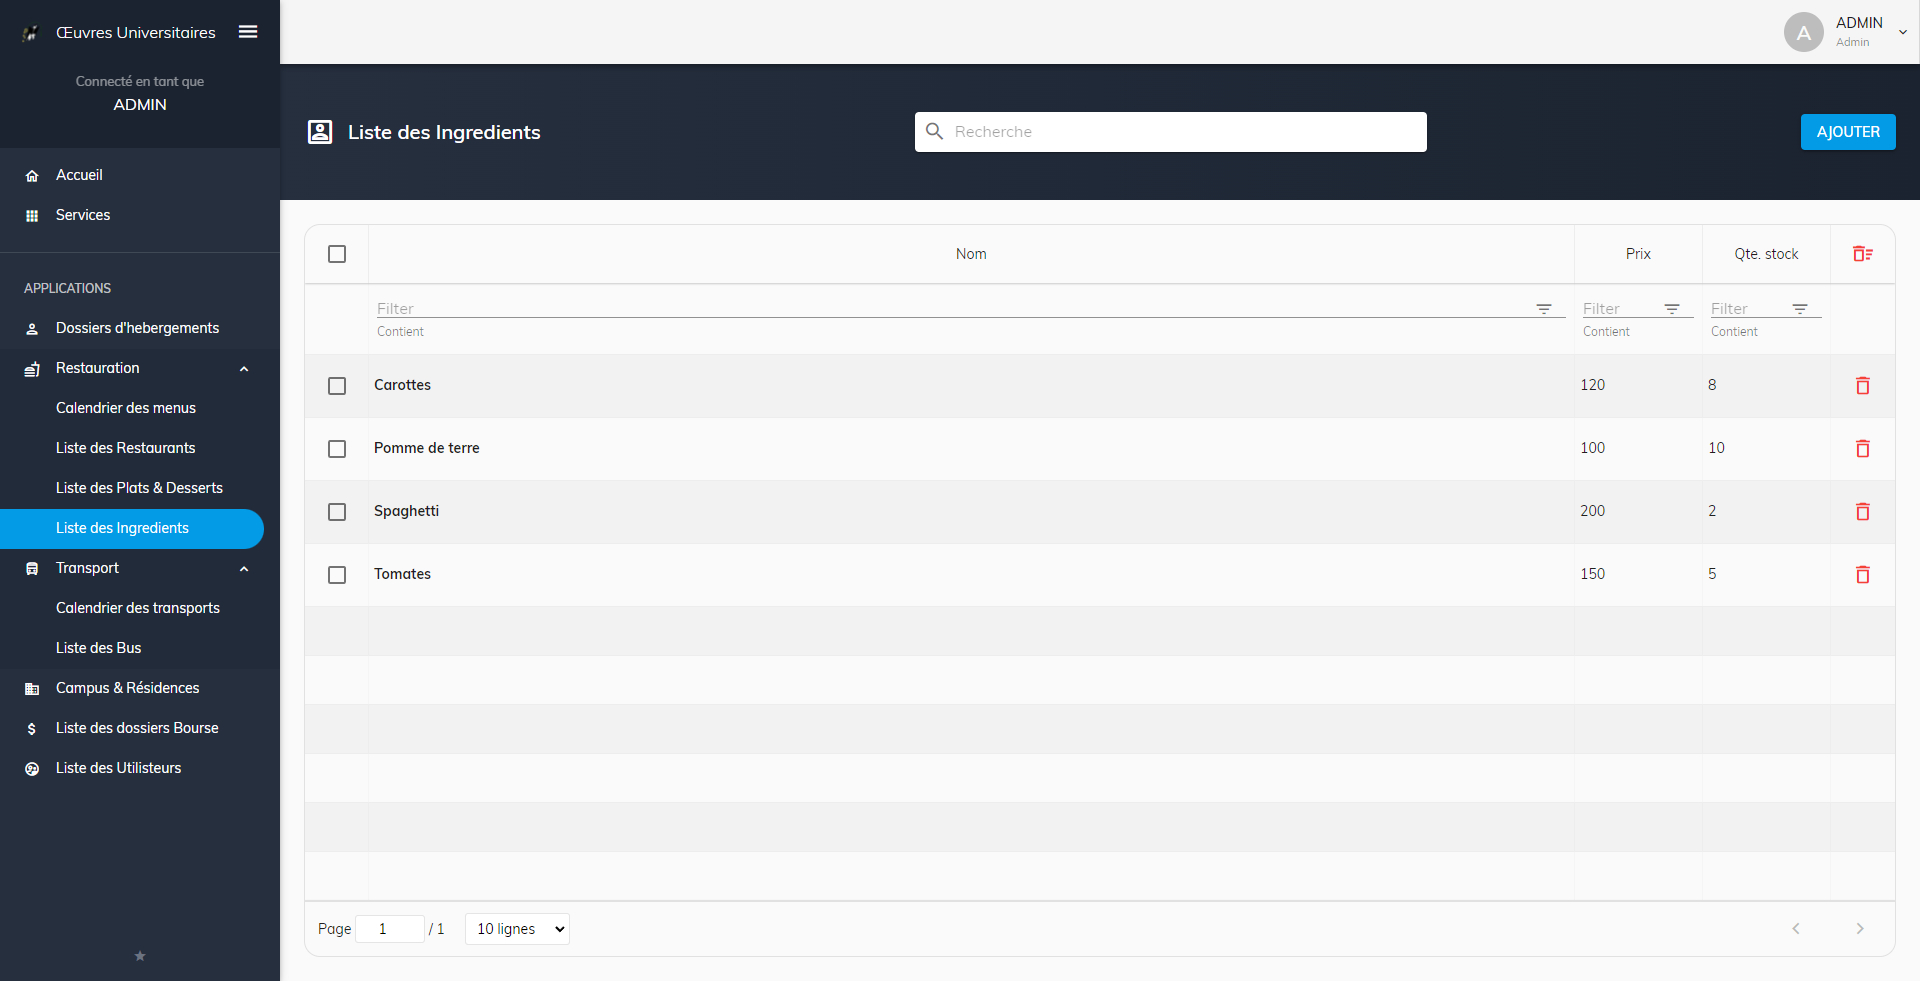
\includegraphics[scale=0.21]{PFE Screens/Admin/Restauration/Ingredients/liste.jpg}
        \caption{Interface utilisateur 'Liste des Ingredients'}
    \end{figure}
    
    \subsection{Interface utilisateur - Détails des menus du mois}
    \begin{figure}[H]
        \centering
        \includegraphics[scale=0.21]{PFE Screens/Admin/Restauration/Calendrier/Détails du moi.jpg}
        \caption{Interface utilisateur - Détails des menus du mois}
    \end{figure}

\section{Conclusion}
Dans ce chapitre nous avons montré l'environnement de travail, les outils utiliser pour créer notre application ainsi que les techniques et les bibliothèques qui nous ont aider dans ce processus.\\

Par la suite, nous avons présenté quelles ques interfaces du rendu final de notre application.\\

Tout en respectant le concept développé lors de l'analyse, nous avons pu réaliser les objectifs fixés.\\